This toolkit requires HRTFs to be stored stored in SOFA format~\citep{AES69-2015}.
The HRTF files contain, among other things, the measured HRIRs and the grid of corresponding measurement positions.
Depending on the decoder used, the HRTFs may need to be interpolated,
and depending on the intended playback system (e.g., type of headphones), the HRTFs may need to be equalized.
Consequently, the SABRE toolkit contains several options for carrying out these processes.

\subsection{Interpolation}
When measured HRTFs are not available at the desired grid positions, interpolation is performed through one of the following methods.

\paragraph*{Nearest Neighbor:} By default, we perform nearest-neighbor interpolation.
This is carried out by minimizing the $\ell^2$ norm (Euclidean distance) between the desired position
$\vec{v}_{q'}$ and each measurement position $\vec{u}_q$.

\paragraph*{Time Domain:} Alternatively, we can perform weighted-average interpolation of the HRIRs for three different interpolation schemes:
natural neighbor, linear, and spherical-harmonic.\footnote{For spherical-harmonic interpolation, the interpolation weights are given as a matrix by $\mathbf{M} = \mathbf{Y}_Q^+ \mathbf{Y}_{Q'}$, where $\mathbf{Y}_Q$ is given by~\eqnref{eq:YMatrix} for all measurement positions and up to some maximum order (by default, $L = 4$), and $\mathbf{Y}_{Q'}$ is the same for all desired positions.}
Generally, for some function $f_q$ measured at positions $\vec{u}_q$, the interpolated values, $f'_{q'}$, for all desired positions $\vec{v}_{q'}$, are given by
\begin{equation}\label{eq:interpolation}
\begin{bmatrix} f'_1 & f'_2 & \cdots & f'_{Q'} \end{bmatrix} =
\begin{bmatrix} f_1 & f_2 & \cdots & f_{Q} \end{bmatrix} \cdot \mathbf{M},
\end{equation}
where each element, $w_{q,q'}$, of $\mathbf{M}$ is the interpolation weight from measurement position $\vec{u}_q$ to the desired position $\vec{v}_{q'}$.
Before interpolating, we first measure the onset delays, $\tau_q^\text{L,R}$, using a 10\% ($-20$~dB) threshold for each impulse response.
We then align all of the impulse responses such that their onsets coincide at the earliest onset, 
and separately store the relative delays, given by
\begin{equation}
d_q^\text{L,R} = \tau_q^\text{L,R} - \min \left( \min_q \tau_q^\text{L},~ \min_q \tau_q^\text{R} \right).
\end{equation}
Then we compute interpolation weights from each measurement position to each desired position and interpolate,
using~\eqnref{eq:interpolation}, the time-aligned impulse responses and the relative delays.
Finally, we introduce the interpolated time delays to each interpolated impulse response.

\paragraph*{Frequency Domain:} We can also interpolate by first decomposing the HRTFs into magnitude spectra and time delays.
The magnitude spectra are given in dB by
\begin{equation}
P_q^\text{L,R}(f) = 10 \log_{10} \left( \left| H_q^\text{L,R}(f) \right|^2 \right),
\end{equation}
where $H$ denotes the Fourier transform of $h$.
We then interpolate the magnitude responses and time delays using~\eqnref{eq:interpolation}.
The interpolated magnitude responses are then converted into minimum-phase impulse responses,
and the interpolated onset delays are introduced to yield the final interpolated HRIRs.

\subsubsection{Interpolation Threshold}
Optionally, we may apply a threshold to determine which desired positions are close enough to a measurement position such that they do not require interpolation.
For each desired position, we find the nearest measurement position and compute the angular distance between the two, given by
\begin{equation}
\psi = \cos^{-1} \left( \frac{\vec{u}_q}{\|\vec{u}_q\|} \cdot \frac{\vec{v}_{q'}}{\|\vec{v}_{q'}\|} \right),
\end{equation}
where $\| \cdot \|$ denotes the $\ell^2$ norm of a vector.
If this angular distance exceeds a user-specified threshold, then the selected interpolation method is carried out.
Otherwise, nearest-neighbor interpolation is used.

\subsection{Equalization}
For optimal binaural playback, one should use individually equalized headphones~\citep{ScharerLindau2009}.
As this may not always be possible, we provide several methods of equalization
so that the user may try to compensate for the equalization of the headphones.
We design the equalization filters using the full set of measured HRTFs
and apply them to the (possibly interpolated) HRTFs for the desired positions.

\paragraph*{None:} By default, the HRTFs are not equalized.
This option should only be used if the playback headphones will be individually equalized on the user's ears.

\paragraph*{Frontal:} For headphones that use frontal-incidence ``free-field'' equalization,
we can equalize all HRTFs by the HRTF pair nearest to $(\theta,\phi) = (0,0)$.
The transfer function of the regularized inverse filter is given by~\citep{Farina2007a}
\begin{equation}\label{eq:A2_SABRE_Toolkit:EQ_Filter}
Z(f) = \frac{H^\ast(f)}{H^\ast(f) H(f) + \beta(f)},
\end{equation}
where $(\cdot)^\ast$ denotes complex conjugation and $\beta$ is a frequency-dependent regularization function.
This function is defined by a set of parameters, which are defined graphically in~\figref{fig:A2_SABRE_Toolkit:Farina_Regularization}, and whose default values are given by
\begin{equation*}
\begin{array}{l l l}
\beta_0 = 10^{-4}, &f_{L0} = 50~\text{Hz}, &f_{H0} = 21~\text{kHz}, \\
\beta_1 = 10^{-2}, &f_{L1} = 20~\text{Hz}, &f_{H1} = 22~\text{kHz}.
\end{array}
\end{equation*}

% Plot of beta profile
\begin{figure}[t]
\centering
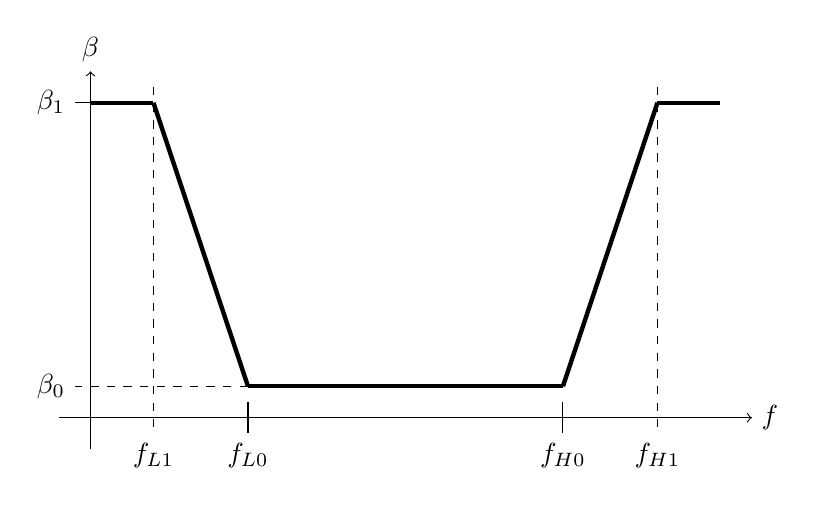
\begin{tikzpicture}[scale=4]
% Parameters
\def\betaone{1}; \def\betazero{0.1};
\def\fzero{0}; \def\fNyq{2};
\def\fLone{0.2}; \def\fLzero{0.5};
\def\fHzero{1.5}; \def\fHone{1.8};

% Axes
\draw[->] (\fzero-0.1,0) -- (\fNyq+0.1,0) node[right]{$f$};
\draw[->] (\fzero,-0.1) -- (\fzero,1.1) node[above]{$\beta$};

% Tick labels
\draw (\fzero+0.05,\betaone) -- (\fzero-0.05,\betaone) node[left]{$\beta_1$};
\draw[dashed] (\fLzero,\betazero) -- (\fzero-0.05,\betazero) node[left]{$\beta_0$};
\draw[dashed] (\fLone,\betaone+0.05) -- (\fLone,-0.05) node[below]{$f_{L1}$};
\draw (\fLzero,0.05) -- (\fLzero,-0.05) node[below]{$f_{L0}$};
\draw (\fHzero,0.05) -- (\fHzero,-0.05) node[below]{$f_{H0}$};
\draw[dashed] (\fHone,\betaone+0.05) -- (\fHone,-0.05) node[below]{$f_{H1}$};

% Plot
\draw[ultra thick] (\fzero,\betaone) -- (\fLone,\betaone);
\draw[ultra thick] (\fLone,\betaone) -- (\fLzero,\betazero);
\draw[ultra thick] (\fLzero,\betazero) -- (\fHzero,\betazero);
\draw[ultra thick] (\fHzero,\betazero) -- (\fHone,\betaone);
\draw[ultra thick] (\fHone,\betaone) -- (\fNyq,\betaone);
\end{tikzpicture}
\caption[Frequency-dependent regularization function for HRTF equalization.]{
Frequency-dependent regularization function of the inverse filters for HRTF equalization.}
\label{fig:A2_SABRE_Toolkit:Farina_Regularization}
\end{figure}

\paragraph*{Diffuse:} For headphones that employ diffuse-field equalization,
we can equalize the HRTFs by the average magnitude spectrum over all directions.
This is computed as the omnidirectional term of the spherical-harmonic decomposition of the HRTF magnitude spectra (in dB),
where the decomposition is computed using the pseudoinverse of $\mathbf{Y}$, given by~\eqnref{eq:YMatrix} for all measurement directions and up to order $L = 4$.
The equalization filter is then computed for the average magnitude spectrum using \eqnref{eq:A2_SABRE_Toolkit:EQ_Filter}.

\paragraph*{Horizontal:} Alternatively, we can compute an average HRTF over all horizontal-plane directions.
The procedure for this is very similar to the diffuse-field equalization, but the average spectrum is computed using only the HRTFs with elevation $|\theta| < 5^\circ$.
The equalization filter is then computed for the average magnitude spectrum using \eqnref{eq:A2_SABRE_Toolkit:EQ_Filter}.